\chapter{$D \rightarrow \pi$ and $B \rightarrow \pi$ form factors}\label{cha:DBtopi}

\section{Correlator fit}\label{sec:Hpi_corrfuncs}
In later stages of this project however we noticed that, on select ensembles, the fit posteriors for this discretization parameter consistently differed from its prior by one or several standard deviations.  This prompted us to apply the standard $\log(\mathrm{GBF})$ testing routine discussed in \ref{sec:prior_determination_methodology} to $P[\epsilon^M]$ uncertainties.  We however halted the $\log(\mathrm{GBF})$ testing when it would have preferred prior uncertainties smaller $\pm1.0$.  This was the case for most most $P[\epsilon^M]$ uncertainties, and so the majority of dispersion parameter priors remain as $P[\epsilon^M] = 0\pm1$.  The most distinct deviation from this norm appears in the fine physical (fphys) ensemble for both the pion and the kaon.  The $\log(\mathrm{GBF})$ preferred uncertainties for $P[\epsilon^{\pi}]$, $P[\epsilon^{K}]$ are $\pm 36.0$ and $\pm50.0$ respectively.  While these uncertainties are relatively large, in test fitting we find that the fphys ensemble fit posteriors for $P[\epsilon^{\pi}]$, $P[\epsilon^{K}]$ have large, greater than one fractional uncertainties, $6(13)$ and $3.0(9.8)$ for example.  Furthermore, such large uncertainties for $P[\epsilon^{\pi}]$, $P[\epsilon^{K}]$ on the fphys ensemble mean that the priors for high twist light meson energies $P[aE^M_{\vec{p}}]$ on that ensemble also have relatively large fractional uncertainties: $0.75-1.0$ for example: this is a consequence of equation \ref{eq:dispersion_energy}.  

The conclusion we come to from these observations is that, on the fphys ensemble, some combination of momentum related discretization effects greatly reduces our ability to set justifiably narrow priors for high twist pion and kaon energies.  Thankfully, the signal from these high twist meson energies is strong enough that in test fitting, despite their broad priors, the posteriors of these energies have fractional uncertainties that range from $0.01-0.04$.  For the $H_s\rightarrow K$ decay exclusively, we also found for the sf5 and sfphys ensembles, $\log(\mathrm{GBF})$ testing preferred $P[\epsilon^{K}]$ uncertainness of $\pm5.0$ and $\pm3.0$ respectively.  In test fitting, the fit posteriors for $\epsilon^{K}$ were both consistent with their priors, and had central values within the range of $0.0\pm1.0$.

\subsection{Results}\label{sec:Hpi_results}
\begin{figure}
    \centering
    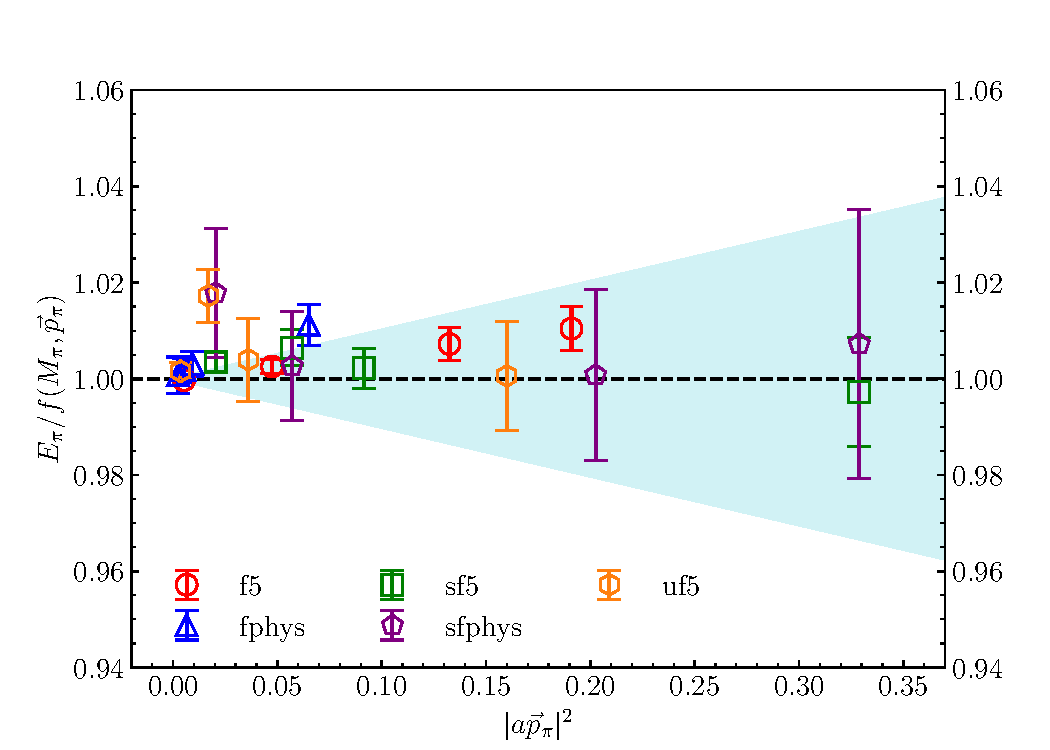
\includegraphics[width=0.8\linewidth]{chapter6/pdfs/customHpi_Edisp_plots.pdf}
    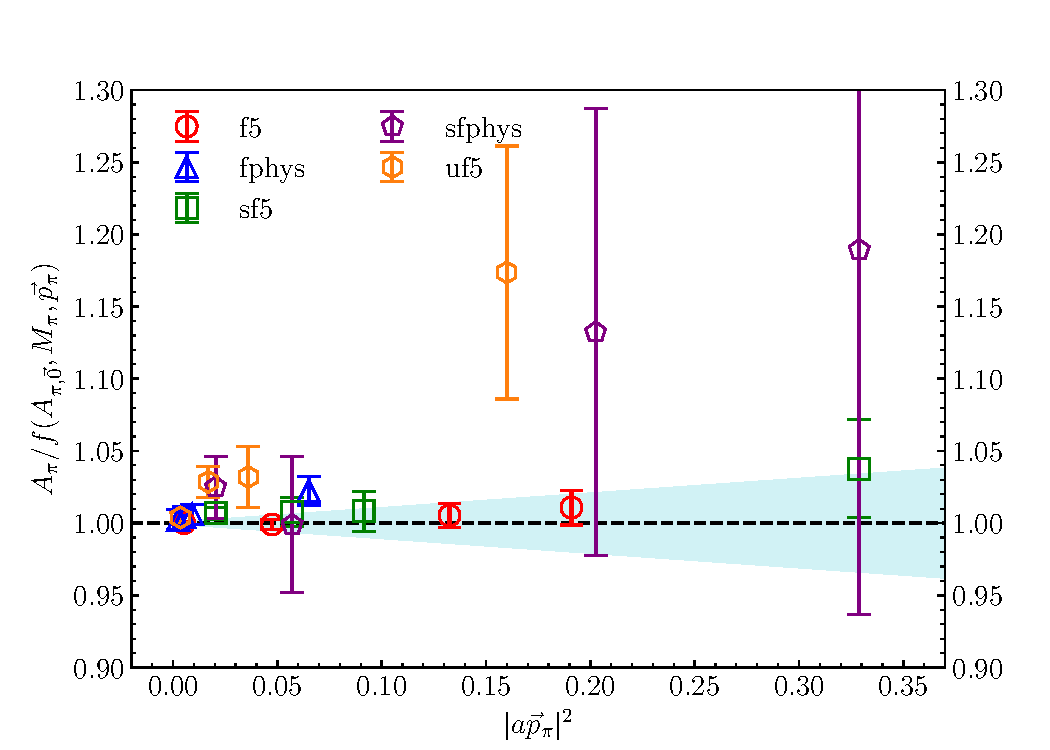
\includegraphics[width=0.8\linewidth]{chapter6/pdfs/customHpi_Ampdisp_plots.pdf}
    \caption{Energy (top) and amplitude (bottom) dispersion relation plots for current set of $H\rightarrow\pi$ correlator fits.  Data shown are ground state, non-zero twist energy and amplitude fit posteriors divided by a function equal to the right hand side of either equation \ref{eq:dispersion_energy} (energy) or equation \ref{eq:dispersion_amplitude} (amplitude) without the discretization factor.  The shaded cyan corresponds to the area bound by the function $y=1\pm \left(\frac{a\vec{p}}{\pi}\right)^2$.}
    \label{fig:Hpi_disp-plots}
\end{figure}

\begin{table*}
\caption{Parameters and statistics related to the correlation functions generated from the gluon field ensembles used in this work.  Column 2 gives the number of correlator configurations $N_\mathrm{cfg}$ times the number of sources $N_\mathrm{src}$ for given ensemble.  Column 3 gives the range of heavy quark masses (in lattice units), where the lightest option is chosen to be tuned to the physical charm quark mass.  Column 4 gives the non-zero twist angles $\theta\neq0.0$, which relate to three-momentum via equation \ref{eq:twist_angle}; we note that all ensembles also have correlators with values of $\theta=0$ as well.  Finally, column 5 gives the range of source-sink separation values $T$.  This table is identical to table \ref{tab:HsK_Stats} in chapter \ref{cha:DsBstoK}, as these parameters and statistics apply to both the $H\rightarrow\pi$ and $H_s\rightarrow k$ meson decays}
\begin{center} 
\begin{tabular}{l c c c c}
\hline
      Set & $N_{\mathrm{cfg}}\times N_{\mathrm{src}}$ & $am_h$ & $\theta\neq0.0$ & $T$ \\
\hline
\hline
    1 - f5   &$500 \times 16$  & 0.450, 0.55, 0.675, 0.8 &  0.4281, 1.282, 2.1410, 2.570 & 15, 18, 21, 24 \\
\hline
    2 - fphys   & $500 \times 8$& 0.433, 0.555, 0.678, 0.8 &  0.58, 0.87, 1.13, 3.000 & 15, 18, 21, 24 \\
\hline
        3 - sf5 & $500 \times 8$& 0.274, 0.5, 0.65, 0.8 &  1.261, 2.108, 2.666, 5.059 & 22, 25, 28, 31 \\
\hline
    4- sfphys &$100 \times 4$& 0.2585, 0.5, 0.65, 0.8 &  2.522, 4.216, 7.94, 10.118 & 22, 25, 28, 31 \\
\hline
    5 - uf5 & $375 \times 4$& 0.194, 0.4, 0.6, 0.8 & 0.706, 1.529, 2.235, 4.705 & 29, 34, 39, 44 \\
\hline
\hline
\end{tabular}
\end{center}
\label{tab:Hpi_Stats}
\end{table*}

\subsection{Priors}\label{sec:Hpi_corr_priors}

\begin{table}[]
    \centering
    \caption{Fractional uncertainties given to priors for ground state meson masses $\Delta(M)$ and amplitudes $\Delta(A)$.  Heavy meson amplitude fractional uncertainties $\Delta(M_H)$ apply only to the lightest $H$ meson option on each ensemble.  The ratio $R(\nicefrac{A_3}{A_0})$ is used in equation \ref{eq:Hmeson_amp_scaling} to determine the fractional uncertainties of of the heavier $H$ meson amplitude priors. $\Delta(A^*)$ is the fractional uncertainty given to all oscillating and or non-ground state amplitude priors.}
    \begin{tabular}{c c c c c c c} 
    \hline
    Ensemble & $\Delta(M_\pi)$ & $\Delta(M_H)$ & $\Delta(A_\pi)$  & $\Delta(A_H)$ & $R(\nicefrac{A_3}{A_0})$ & $\Delta(A^*)$\\
    \hline
    f5 & 0.05 & 0.05 & 0.05 &  0.11 &  2.0 & 5.0\\
    fphys & 0.10 & 0.05 & 0.05 & 0.22 & 2.0 & 6.1\\
    sf5 & 0.10 & 0.05 & 0.10 & 0.10 & 4.0 & 2.6\\
    sfphys & 0.60 & 0.10 & 0.30 & 0.65 & 2.0 & 2.0\\
    uf5 & 0.25 & 0.05 & 0.20 & 0.20 & 4.0 & 2.0\\
    \hline
    \end{tabular}
    \label{tab:Hpimeson_mass_and_amp_priors}
\end{table}

\begin{table}[]
    \centering
    \caption{$H\rightarrow\pi$ ground state three-point amplitude priors $P[J_{00}^{nn}]$ for all ensembles, twists $\theta$, and currents $J \in \{S,V^0,V^1,T\}$.  Twist is related to the pion's three-momentum $\vec{p}$ via equation \ref{eq:twist_angle}.  Methods for determining these priors is discussed in section \ref{sec:Amp_effs_3pt}.}
    \label{tab:3ptpriors_Hpi}
    \begin{tabular}{c c | c c c c}
    \hline
    \hline
    Ensemble & $\theta$ & $S$ & $V^0$ & $V^1$ & $T$ \\
    \hline
    \hline
    f5 & 0.0 & 2.6(2.6) & 1.0(1.0) & - & - \\
       & 0.4281 & 2.4(2.4) & 0.9(0.9) & 0.15(0.15) & 0.1(0.1)\\
       & 1.282 & 1.5(1.5) & 0.6(0.6) & 0.22(0.22) & 0.15(0.15)\\
       & 2.1410 & 1.0(1.0) & 0.5(0.5) & 0.2(0.2) & 0.12(0.12)\\
       & 2.570 & 0.8(0.8) & 0.4(0.4) & 0.2(0.2) & 0.13(0.13)\\
    \hline
    fphys & 0.0 & 4.75(4.75) & 3.0(3.0) & - & - \\
          & 0.58 & 3.75(3.75) & 2.5(2.5) & 0.2(0.2) & 0.15(0.15)\\
          & 0.87 & 3.25(3.25) & 2.0(2.0) & 0.25(0.25) & 0.18(0.18)\\
          & 1.13 & 2.75(2.75) & 1.5(1.5) &0.3(0.3) & 0.15(0.15)\\
          & 3.000 & 1.50(1.50) & 0.75(0.75) & 0.25(0.25) & 0.15(0.15)\\
          & 5.311 & 0.5(0.5) & 0.25(0.25) & 0.15(0.15) & 0.1(0.1)\\
    \hline
    sf5   & 0.0   & 2.5(2.5)   & 2.0(2.0)   & -          & -       \\    
          & 1.261 & 1.75(1.75) & 1.0(1.0)   & 0.3(0.3)   & 0.2(0.2)\\ 
          & 2.108 & 1.25(1.25) & 0.65(0.65) & 0.25(0.25) & 0.2(0.2)\\
          & 2.666 & 1.0(1.0)   & 0.6(0.6)   & 0.25(0.25) & 0.2(0.2)\\
          & 5.059 & 1.0(5.0)   & 1.0(4.0)   & 1.0(4.0)   & 0.2(3.0)\\
    \hline
    sfphys & 0.0    & 4.75(4.75) & 4.0(4.0)   & -          & - \\ 
           & 2.522  & 1.75(1.75) & 1.25(1.25) & 0.35(0.35) & 0.2(0.2)\\ 
           & 4.216  & 1.5(1.5)   & 1.0(1.0)   & 0.35(0.35) & 0.25(0.25)\\ 
           & 7.94   & 1.0(1.5)   & 0.5(1.0)   & 0.3(0.3)   & 0.2(0.2)\\
           & 10.118 & 1.0(3.0)   & 0.5(2.0)   & 0.3(1.0)   & 0.2(1.0)\\
    \hline
    uf5 & 0.0   & 2.75(2.75) & 2.0(2.0)   & -          & - \\
        & 0.706 & 2.25(2.25) & 1.5(1.5)   & 0.25(0.25) & 0.2(0.2) \\
        & 1.529 & 1.5(1.5)   & 1.0(1.0)   & 0.3(0.3)   & 0.20(0.2) \\
        & 2.235 & 1.0(1.0)   & 0.75(0.75) & 0.3(0.3)   & 0.20(0.2) \\
        & 4.705 & 1.0(1.0)   & 1.0(2.0)   & 0.3(1.0)   & 0.2(0.5)\\
    \hline
    \hline
    \end{tabular}
\end{table}

\begin{table}
  \caption{$H\rightarrow\pi$ prior absolute uncertainties for all ensembles, for all oscillating and or non-ground state fit parameters $J_{ij}^{kl} \neq J_{00}^{oo}$, for $J\in \{S,V^0,V^1,T\}$.  The notation $J_{\neq0}$ indicates the values used to assign priors to all higher order exponential states $J_{ij\neq00}^{kl}$. The notation $J_{\mathrm{osc}}$ indicates the values used to assign priors to all lowest lying oscillating states $J_{00}^{kl\neq nn}$. Central values given to all associated priors are equal to 0.0. A special prior uncertainty scaling term $\sigma_\mathrm{ens}$ for each ensemble is given in final column.  The scaling term applies to select non-ground state three point amplitudes $J_{00}^{on}$ and $J_{10}^{kl}$ for all $k,l \in \{n,o\}$.}
  \begin{center} 
    \begin{tabular}{l c c c c c c c c c}
    \hline
    \hline
    Ensemble & $S_{\neq 0}$ & $S_{\mathrm{osc}}$ & $V^0_{\neq 0}$ & $V^0_{\mathrm{osc}}$ & $V^1_{\neq 0}$ & $V^1_{\mathrm{osc}}$ & $T_{\neq 0}$ & $T_{\mathrm{osc}}$ & $\sigma_\mathrm{ens}$\\
    \hline
    \hline
    f5 & 0.5 & 1.75 & 0.7 & 3.5 & 0.1 & 0.22 & 0.07 & 0.12 & 1.8\\
    fphys & 1.43 & 4.4 & 1.0 & 10.0 & 0.21 & 0.06 & 0.08 & 0.12 & 2.2\\
    sf5 & 0.32 & 1.4 & 0.46 & 3.0 & 0.10 & 0.23 & 0.05 & 0.25 & 4.0\\
    sfphys & 0.45 & 3.0 & 0.55 & 5.0 & 0.04 & 0.5 & 0.04 & 0.07 & 5.5\\
    uf5 & 0.30 & 0.60 & 0.32 & 3.0 & 0.04 & 0.08 & 0.04 & 0.07 & 5.0\\
    \hline
    \hline
    \end{tabular}
    \end{center}
  \label{tab:3pt_pesky_priors_Hpi}
\end{table}


\section{$z$-expansion fit}\label{sec:Hpi_zfit}

\subsection{Priors}\label{sec:Hpi_zfit_priors}

\subsection{Results}\label{sec:Hpi_zfit_results}

\section{Status of form factors calculations}\label{sec:Hpi_FF_status}

\subsection{$D\rightarrow\pi$}\label{sec:Dpi_status}

\subsection{$B\rightarrow\pi$}\label{sec:Hpi_status}